\begin{frame}[t, fragile]{Pandas Series}
  \begin{block}{Definição}
    Objeto que representa uma estrutura de dados unidimensional similar ao array mas com algumas características a mais.
  \end{block}
  \begin{columns}
    \begin{column}{0.5\textwidth}
        \begin{itemize}
          \item Composta por dois arrays:
          \item (i) dados
          \item (ii) índice
        \end{itemize}
    \end{column}

    \begin{column}{0.5\textwidth}
      \begin{center}
        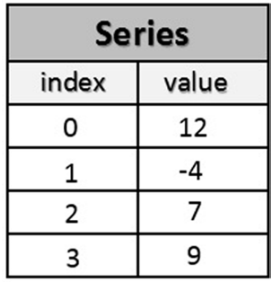
\includegraphics[scale=.40]{aula-2/figuras/pandas-series-1.png}
      \end{center}
    \end{column}
  \end{columns}
\end{frame}
%
\begin{frame}[t, fragile, allowframebreaks]{Declarando uma Serie}
  \begin{itemize}
    \item Índice padrão
  \end{itemize}
  \lstinputlisting[language=python]{aula-2/codigos/pandas/pandas-series-1.py}  
  \framebreak
  \begin{itemize}
    \item Índice personalizado
  \end{itemize}
  Livro: O Perfil das Empresas Brasilieiras em Gestão e Governança de Dados
  \lstinputlisting[language=python]{aula-2/codigos/pandas/pandas-series-2.py}  
\end{frame}
\begin{frame}[t, fragile]{Acessando índices e valores}
  \lstinputlisting[language=python]{aula-2/codigos/pandas/pandas-series-3.py}  
\end{frame}
%
\begin{frame}[t, fragile]{Selecionando valores em uma Serie}
  \lstinputlisting[language=python]{aula-2/codigos/pandas/pandas-series-4.py}  
\end{frame}
%
\begin{frame}[t, fragile]{Atribuindo valores}
  \lstinputlisting[language=python]{aula-2/codigos/pandas/pandas-series-5.py}  
\end{frame}
%
\begin{frame}[t, fragile]{Filtrando valores}
  \lstinputlisting[language=python]{aula-2/codigos/pandas/pandas-series-6.py}  
\end{frame}
%
\begin{frame}[t, fragile, allowframebreaks]{Avaliando valores}
  \lstinputlisting[language=python]{aula-2/codigos/pandas/pandas-series-7.py}  
\end{frame}
%
